\documentclass[twocolumn]{article}
\usepackage[T1]{fontenc}
\usepackage{lmodern}
\usepackage{amssymb,amsmath}
\usepackage{ifxetex,ifluatex}
\usepackage{fixltx2e} % provides \textsubscript
% use microtype if available
\IfFileExists{microtype.sty}{\usepackage{microtype}}{}
\ifnum 0\ifxetex 1\fi\ifluatex 1\fi=0 % if pdftex
  \usepackage[utf8]{inputenc}
\else % if luatex or xelatex
  \usepackage{fontspec}
  \ifxetex
    \usepackage{xltxtra,xunicode}
  \fi
  \defaultfontfeatures{Mapping=tex-text,Scale=MatchLowercase}
  \newcommand{\euro}{€}
\fi
% Redefine labelwidth for lists; otherwise, the enumerate package will cause
% markers to extend beyond the left margin.
\makeatletter\AtBeginDocument{%
  \renewcommand{\@listi}
    {\setlength{\labelwidth}{4em}}
}\makeatother
\usepackage{enumerate}
\usepackage{graphicx}
% We will generate all images so they have a width \maxwidth. This means
% that they will get their normal width if they fit onto the page, but
% are scaled down if they would overflow the margins.
\makeatletter
\def\maxwidth{\ifdim\Gin@nat@width>\linewidth\linewidth
\else\Gin@nat@width\fi}
\makeatother
\let\Oldincludegraphics\includegraphics
\renewcommand{\includegraphics}[1]{\Oldincludegraphics[width=\maxwidth]{#1}}
\ifxetex
  \usepackage[setpagesize=false, % page size defined by xetex
              unicode=false, % unicode breaks when used with xetex
              xetex]{hyperref}
\else
  \usepackage[unicode=true]{hyperref}
\fi
\hypersetup{breaklinks=true,
            bookmarks=true,
            pdfauthor={},
            pdftitle={},
            colorlinks=true,
            urlcolor=blue,
            linkcolor=magenta,
            pdfborder={0 0 0}}
\setlength{\parindent}{0pt}
\setlength{\parskip}{6pt plus 2pt minus 1pt}
\setlength{\emergencystretch}{3em}  % prevent overfull lines
\setcounter{secnumdepth}{4}

\author{}
\date{}

\begin{document}

\title{Testing Parts for Phys1600}
\author{Dan Peirce B.Sc.}
\date{Dokuwiki version created October 2012 \\ converted to latex/pdf on August 3, 2013 \\ revised August 06, 2013}

\maketitle
\tableofcontents


\section{Related Pages}

\begin{itemize}
\item
  pic18lf\_sound\_project\footnote{\url{http://www3.telus.net/danpeirce/notes/pic18lf_sound_project.html}} -- moved
  some ``other things of interest'' not related to sound from that page
  to this page.
\item
  Bitbucket repository pic18\_serial\_io\footnote{\url{https://bitbucket.org/danpeirce/pic18_serial_io}} -- some basic
  code for testing the serial/USB interface is on that public page --
  branches of the project related to specific projects has not been
  added to that repository.
\item
  hello33\footnote{\url{http://www3.telus.net/danpeirce/notes/hello33.html}} even more basic code used to test the USB
  to UART bridge.
\end{itemize}


\section{The Parts}

\begin{enumerate}[1.]
\item
  PIC18LF2620\footnote{\url{http://ww1.microchip.com/downloads/en/devicedoc/39626b.pdf}}
\item
  uUSB-MB5\footnote{\tiny{\url{http://www.abra-electronics.com/products/\%CE\%BCUSB\%252dMB5-Breakout-Board-for-CP2102-mini-USB-to-Serial-.html}}}
  -- this board comes fully assembled as shown.
  (note on driver\footnote{\url{http://www3.telus.net/danpeirce/notes/usb_mb5.html}})
\item
  PICkit3\footnote{\url{http://www.microchip.com/stellent/idcplg?IdcService=SS\_GET\_PAGE\&nodeId=1406\&dDocName=en538340\&redirects=pickit3}}
\item
  Digikey Part number CTX743-ND\footnote{\url{http://www.digikey.ca/product-detail/en/MXO45HS-3C-8M0000/CTX743-ND}}
\end{enumerate}

The uUSB-MB5 provides 3.3Vdc to the PIC18LF2620. The uUSB-MB5 has an
on-board 3.3V regulator which converts the USB supplied nominal 5 V to
the regulated 3.3volts. The regulator also provides short circuit and
thermal protection. It can supply a maximum of 100 mA.

\section{Important Note Regarding Using an Oscilloscope when using
the uUSB-MB5}

In APSC1299 the output of the power supply used floats relative to earth
ground as long as the PICkit2 is not attached to the circuit. When the
uUSB-MB5 is used power comes from the computer USB port. With a desktop
computer the negative side of the supply does not float relative to
ground. It is grounded. The oscilloscope ground clip is also grounded.
Connected the oscilloscope ground clip to anything but the USB ground
will cause a short circuit.

The situation is different when using a laptop powered from the battery.
In this case the negative side of the supply is floating relative to
earth ground. I tested one laptop with the charging power supply plugged
in and found the USB ground was still floating.

\section{Using an External Oscillator}

More than one variant of the supply wiring has been tested.

Figure~\ref{osc8mhz} shows a CTX743-ND on a breadboard. It is a five volt oscillator. In this variant of the wiring the
positive rail at the bottom of the solderless breadboard is used for 5 V
and the positive rail at the top of the breadboard is used for 3.3
volts.

\begin{figure}[htbp]
\centering
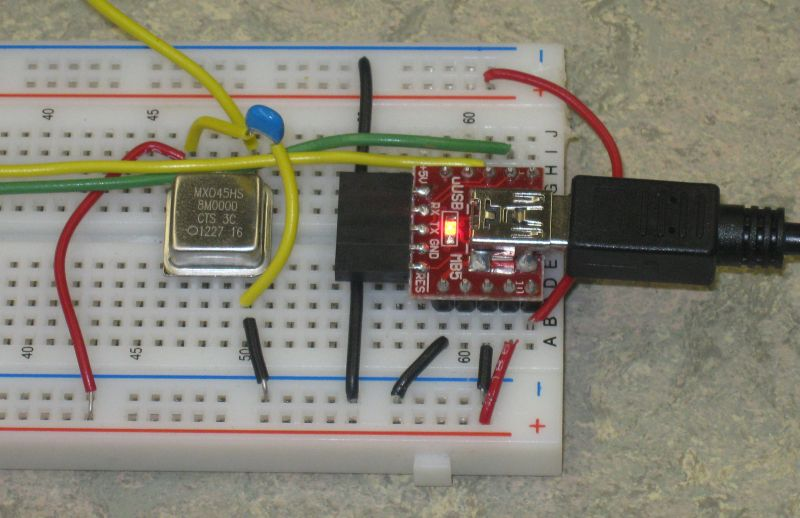
\includegraphics{phys1600/usb-mb5_8mhzosc.jpg}
\caption{The CTX743-ND Oscillator on Breadboard}
\label{osc8mhz}
\end{figure}

Figure~\ref{osc8mhzwideview} shows the complete breadboard in a wider view but is the same circuit as Figure~\ref{osc8mhz}.

\begin{figure}[htbp]
\centering
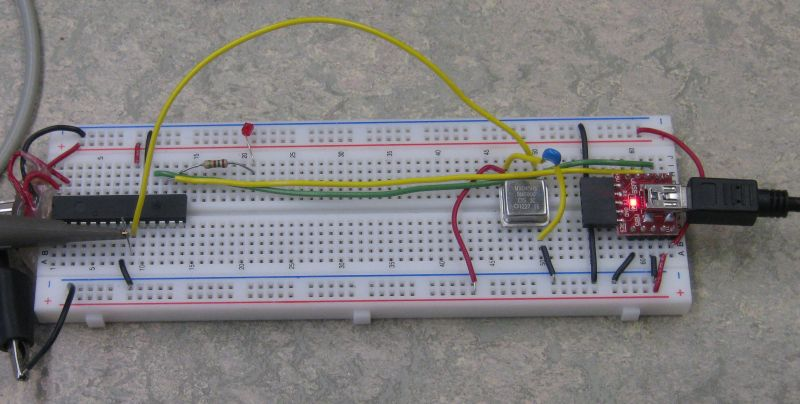
\includegraphics{phys1600/pic_usb-mb5_8mhzosc.jpg}
\caption{Wider View of CTX743-ND on Breadboard}
\label{osc8mhzwideview}
\end{figure}

Note that the PIC is tolerant of 5 volt inputs when powered at 3.3
volts! \textbf{For student use the jumper wire from 5 volts out of the
USB-MB5 could to the nearby power rail could be replaced by a 400 mA
axial leaded fuse.}

\subsection{Alternate Layout for 5 volt Bus}

The circuit in Figures~\ref{osc8mhz} and \ref{osc8mhzwideview} have the 3.3 volt rail as the positive rail at the top of the board and the +5 volt rail as the positive rail at the bottom of the board. Rather then use the lower supply rail for 5 volts an alternative is to
use just one internal row for 5 volts and keep both positive rails at 3.3 volts.
We would like to minimize the use of the raw 5 volts. This is shown in Figure~\ref{osc8mhzalternate}

\begin{figure}[htbp]
\centering
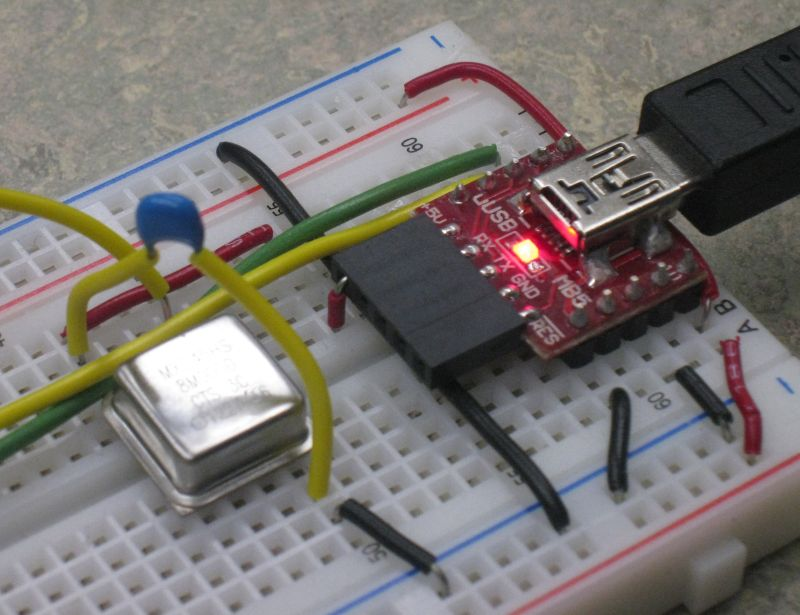
\includegraphics{phys1600/alternative_5v_row2.jpg}
\caption{Alternate Layout for 5 volt Supply (coming out of connector of breakout board)}
\label{osc8mhzalternate}
\end{figure}

\subsection{Oscillator on Protoboard for Short Signal Path}

Since the oscillator is at an RF frequency it is a good idea to keep the
lead short. Building the oscillator on a little piece of protoboard
facilitates this. This can be seen in Figure~\ref{osc8mhzproto}.

\begin{figure}[htbp]
\centering
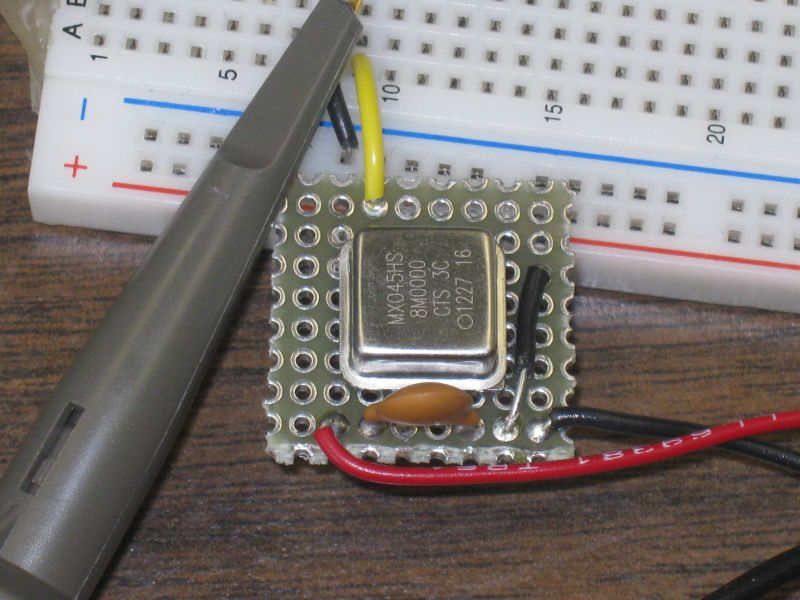
\includegraphics{phys1600/osc_proto.jpg}
\caption{8 MHz Oscillator on Proto-Board}
\label{osc8mhzproto}
\end{figure}

Figure~\ref{osc8mhzprotopic} shows the connection between the PIC and oscillator.

\begin{figure}[htbp]
\centering
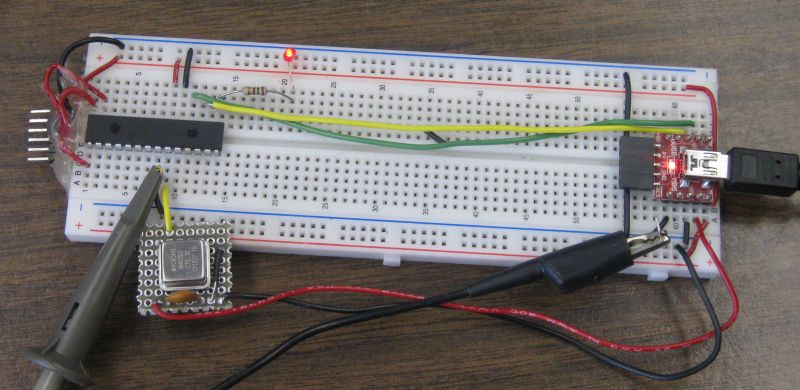
\includegraphics{phys1600/osc_proto_pic.jpg}
\caption{Oscillator Proto-Board Mounted Near PIC}
\label{osc8mhzprotopic}
\end{figure}

\subsection{Oscillator Protoboard Vertical for Even Shorter Signal
Path}

\begin{figure}[htbp]
\centering
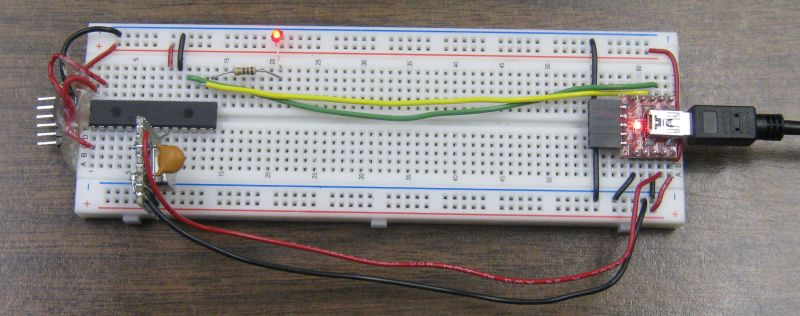
\includegraphics{phys1600/osc_proto_vert.jpg}
\caption{Vertical Oscillator Proto-Board}
\label{osc8mhzprotopicvert}
\end{figure}

\begin{figure}[htbp]
\centering
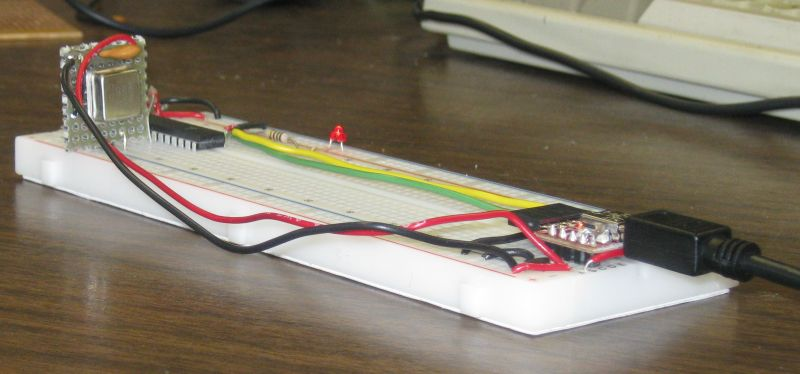
\includegraphics{phys1600/osc_proto_pic_vert.jpg}
\caption{Side View of Vertical Oscillator Proto-Board}
\label{osc8mhzprotopicvertside}
\end{figure}

The conductor between the oscillator output and the osc1 input of the PIC can be made shorter still if the oscillator board is mounted vertically as shown in Figures~\ref{osc8mhzprotopicvert} and \ref{osc8mhzprotopicvertside}.

\subsection{Signal from Oscillator}

Signal from Oscillator when loaded by PIC is shown in Figure~\ref{osc8mhzsignaldso}. The external
oscillator can be used when very precise time measurements are to be
made. The oscillator signal is not an idealized square wave but contains some overshoot on the trailing edge of sharp transitions.

The internal oscillator is quite adequate for many applications.

\begin{figure}[htbp]
\centering
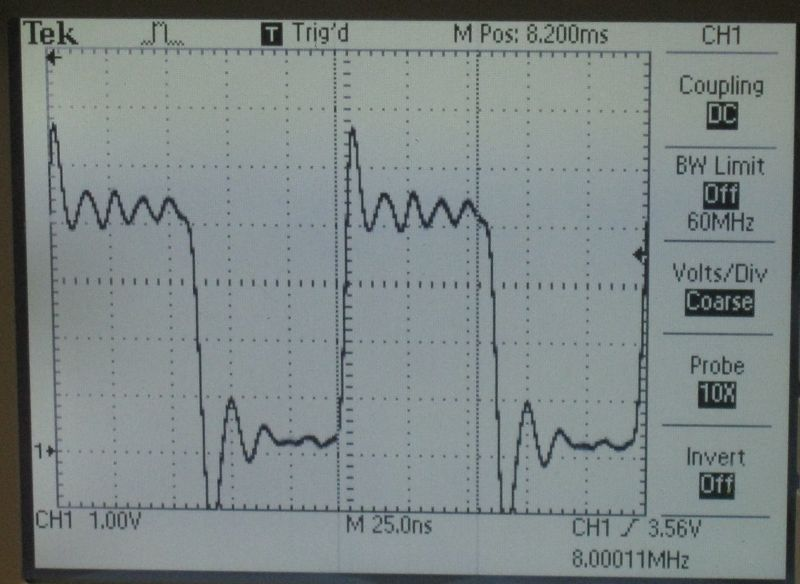
\includegraphics{phys1600/input_to_osc1_pic.jpg}
\caption{8MHz Signal Shown on DSO}
\label{osc8mhzsignaldso}
\end{figure}

\subsection{New Branch on bitbucket repository}

I created a new branch on my git bitbucket repository to reflect the use
of an external oscillator.

\begin{itemize}
\item
  \url{https://bitbucket.org/danpeirce/pic18\_serial\_io/diff/USARTfunc.c?diff2=9517adf437b4\&at=ext\_osc}
\end{itemize}


\section{Without an External Oscillator}

Figure~\ref{pic18lf2620usbmb5} shows the connection between a PIC18LF2620 and a USB-MB5 without an External Oscillator. In this case the PIC oscillator signal is not available. The oscillator divided by four frequency is available on the OSC2 pin.

\begin{figure}[htbp]
\centering
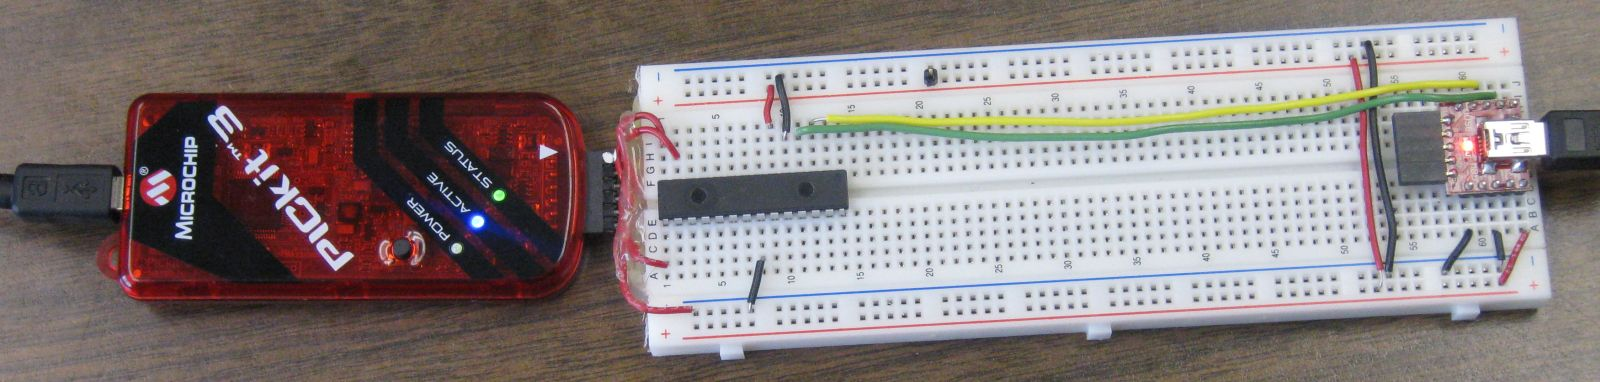
\includegraphics{phys1600/pic18lf2620_usbmb5_pickit3.jpg}
\caption{PIC18LF2620 USB-mb5 PICkit3}
\label{pic18lf2620usbmb5}
\end{figure}

\section{The USB-MB5 for Serial Communication}

The USB-MB5 provides power to the breadboard and it also provides serial communication to the computerhost. Figure~\ref{usbmb5} is a closeup of the wiring to the USB-MB5. The green and yellow wires are for serial communication between the PIC and the USB-MB5.

\begin{figure}[htbp]
\centering
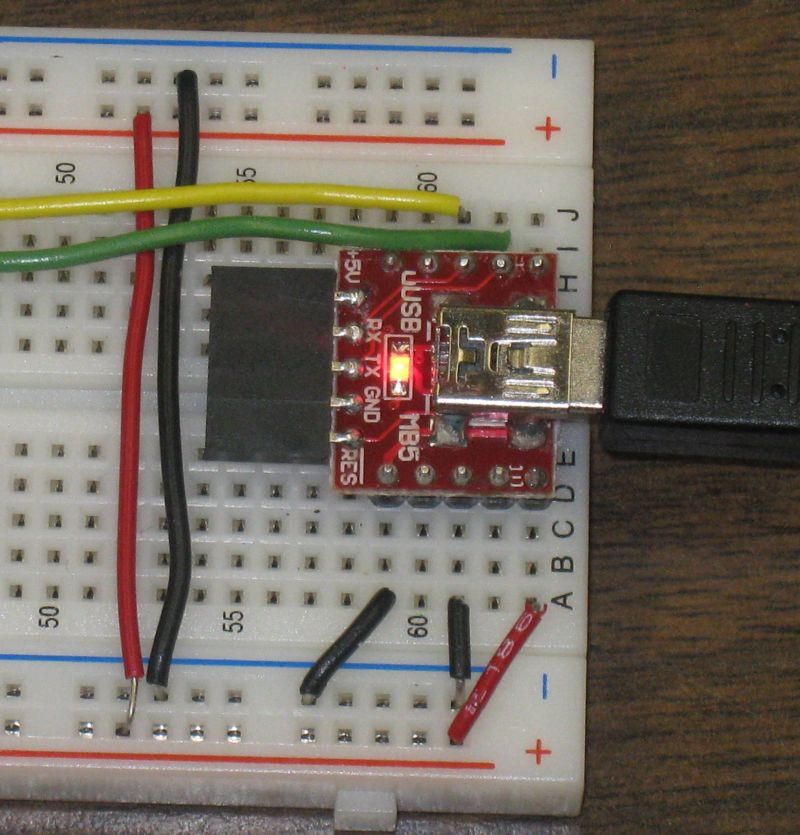
\includegraphics{phys1600/usb-mb5.jpg}
\caption{USB-MB5}
\label{usbmb5}
\end{figure}

In this case I have not used the 5 volt output from the USB-MB5.

\subsection{PIC Test Program}

Made use of existing program
\textbf{pic18\_serial\_io\footnote{\url{https://bitbucket.org/danpeirce/pic18/serial/io}}}.
That project was written for the PIC with interacting with a Raspberry
Pi in mind but it will interact with a Windows PC just as well (see Figure~\ref{putty}).
\begin{figure}[htbp]
\centering
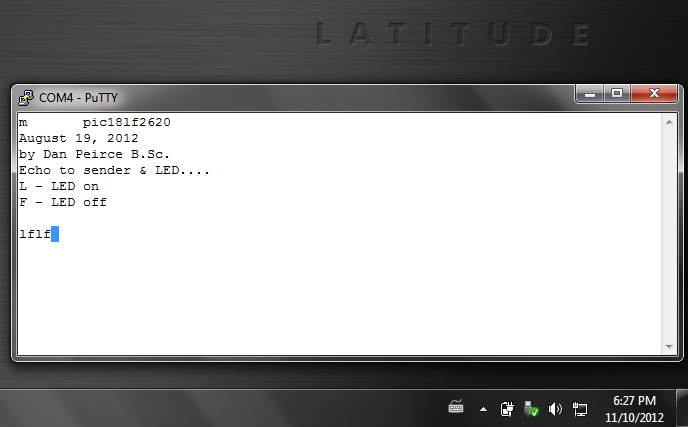
\includegraphics{phys1600/putty_laptop_desktop.png}
\caption{Terminal Window on a Laptop Desktop}
\label{putty}
\end{figure}

Currently this PIC program recognizes three commands.

\begin{enumerate}[1.]
\item
  ``M'' -- sends a menu message - this was used for the test.
\item
  ``L'' -- intended to turn on an LED.
\item
  ``F'' -- intended to turn off an LED.
\end{enumerate}

Note that to test the ``L'' and ``F'' commands a 200 ohm resistor should
be connected to pin 15 of the PIC and the other end of the resistor
should connect to the anode of a LED. The cathode of the LED is
connected to ground.

The PIC will also echo any character it receives back over the serial
link for a loop-back test. If it receives a `\textbackslash{}r' it will add a `\textbackslash{}n'. see
\url{https://bitbucket.org/danpeirce/pic18_serial_io/src/b8c10af1b10d/commands.c}

Complete set of project files can be obtained from
\url{https://bitbucket.org/danpeirce/pic18_serial_io/get/b8c10af1b10d.zip}.

Within these files the header file p18f2620.h is used. There is no
p18lf2620.h file but from a the programming point of view the devices
are equivalent. Also, when the project wizard was used to create the
project file the PIC18F2620 device was selected. The resulting HEX file
is still suitable for the PIC18LF2620.

\subsection{Computer Terminal Program}

On Windows XP I used hyperterminal. Windows 7 does not ship with
hyperterminal.

I tested PuTTY\footnote{\url{http://www.putty.org/}}.

I have been using PuTTY as a SSH client but it also works as a simple
serial terminal.

Figure~\ref{putty} is a screen shot shows a PuTTY session connected to the PIC18LF2620 via
the USB to serial bridge uUSB-MB5.

Note that the PuTTY terminal screen will be empty until something is
typed on the computer (laptop). What ever is typed will be echoed to the
screen (by the PIC) if everything is set-up correctly. Typing ``m''
sends the menu message (from the PIC). Figure~\ref{putty} shows part of the desktop.

\subsubsection{PuTTY Settings}

The following screen shots show the PuTTY settings:

\textbf{PuTTY -\textgreater{} Connection -\textgreater{} Serial} see Figure~\ref{puttyserial}

\begin{figure}[htbp]
\centering
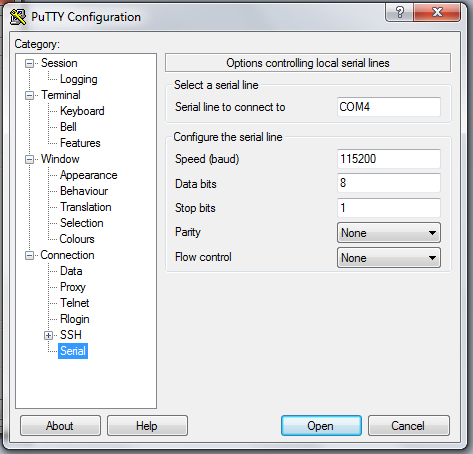
\includegraphics{phys1600/putty_connection.png}
\caption{PuTTY Serial Setting}
\label{puttyserial}
\end{figure}

\textbf{PuTTY -\textgreater{} Window -\textgreater{} Colours}\\Select
\textbf{Use System Colours} to avoid getting white on black. See Figure~\ref{puttycolours}
\begin{figure}[htbp]
\centering
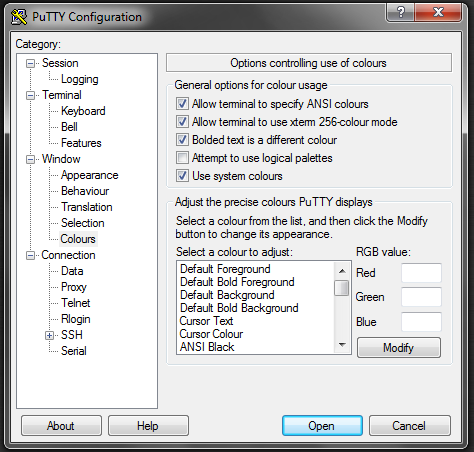
\includegraphics{phys1600/putty_window_colours.png}
\caption{PuTTY Window Colours}
\label{puttycolours}
\end{figure}

\textbf{PuTTY -\textgreater{} Session} (Connection type must be selected
as \textbf{Serial}  See~Figure~\ref{puttysession})
 
\begin{figure}[tbp]
\centering
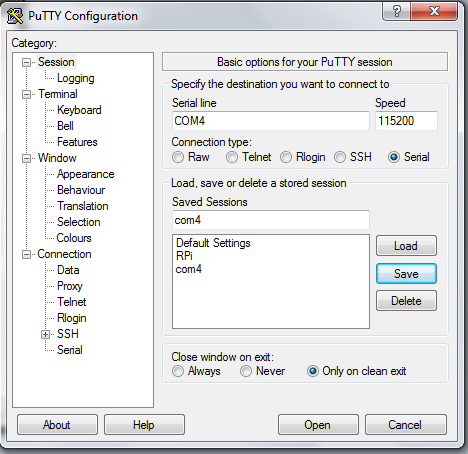
\includegraphics{phys1600/putty_session.png}
\caption{PuTTY Session (serial settings)}
\label{puttysession}
\end{figure}

\section{Getting the PICkit3 to work with the PIC18LF2620}

\subsection{With PICkit3 Pin 2 to 3.3 Volt Connection}

Please note that when this was tested the connections between the
PICkit3 and the PIC18LF2620 were as shown in Figure~\ref{pickit3wiring}.

\begin{figure}[htbp]
\centering
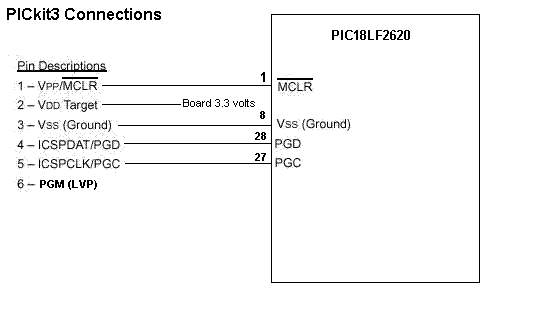
\includegraphics{phys1600/pickit3_connections.png}
\caption{Wiring Between PICkit3 and PIC18LF2620}
\label{pickit3wiring}
\end{figure}

\begin{figure}[htbp]
\centering
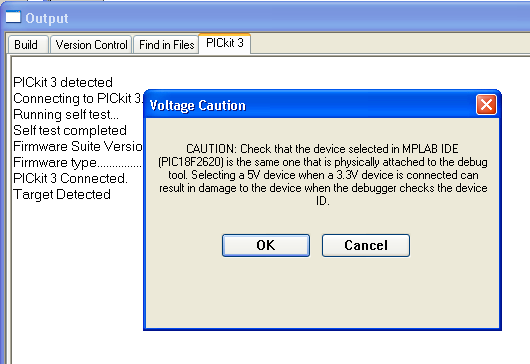
\includegraphics{phys1600/pickit3_on_connect.png}
\caption{Warning Message: Click OK}
\label{warningok}
\end{figure}

Once the \textbf{OK} is selected (Figure~\ref{warningok}) the device ID will be shown:

\begin{verbatim}
      Device ID Revision = 00000007
\end{verbatim}

It is possible to read the source voltage with the PICkit3 and display the result in a MPlab IDE window (see Figure~\ref{readingvoltage}).

\begin{figure}[htbp]
\centering
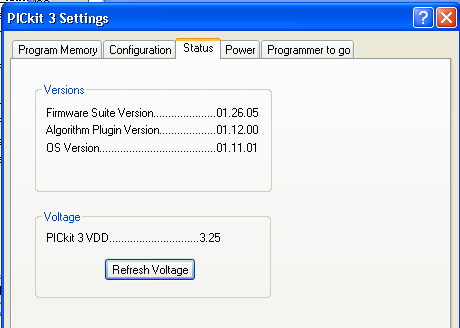
\includegraphics{phys1600/pickit3_reading_voltage.png}
\caption{Reading Voltage With PICkit3}
\label{readingvoltage}
\end{figure}

If the PICkit3 pin2 is connected to the circuit and the circuit is
powered from the USB connection it is essentially that Powering from the
PICkit3 is not checked on the power tab!

\subsection{With PICkit3 Pin 2 Left No Connection}

With the PICkit2 we left the power connection open because we did not
plan to power the board from the PICkit2 and it seemed to avoid the
possible issue of someone inadvertently powering the board from the
PICkit2. With the PICkit3 we still don't want to power our board from
the PICkit3 (and risk damage to it). It appears that with the PICkit3 it
would not be easy to power the board from the PICkit3 unintentionally
and as shown below leaving PIN2 open leads to many extra steps being
necessary. \textbf{This part is included for completeness -- For the
PICkit3 I recomend adding the wire from PIN2 to VDD.}

Note that a PICkit2 will attempt to read the voltage on its pin2. If no
voltage is pressent the firmware will assume that the target needs to be
powered from the PICkit2's supply. It appears that the firmware on the
PICkit3 is different. If no voltage is sensed on pin2 it will give the
following error: (also shown in Figure~\ref{errormsg})

{\footnotesize
\begin{verbatim}
PK3Err0045: You must connect a target device to use PICkit3.
\end{verbatim}
}


Perhaps a better error message would have said that no voltage was
detected. One could use a wire from the board positive rail to the
PICkit3 pin2 or one could use the following procedure which I worked out
by trial and error.

\textbf{The error:} (see Figure~\ref{errormsg})

\begin{figure}[htbp]
\centering
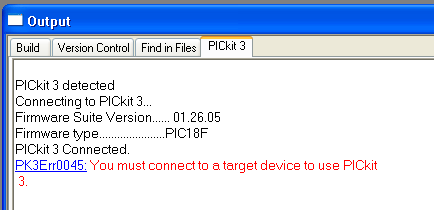
\includegraphics{phys1600/error_on_connect.png}
\caption{The Error Message}
\label{errormsg}
\end{figure}

Select \textbf{Programmer -\textgreater{} Settings} (see Figure~\ref{programmersettings}

\begin{figure}[htbp]
\centering
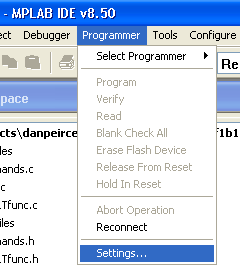
\includegraphics{phys1600/programmer_settings.png}
\caption{Finding Programmer Settings}
\label{programmersettings}
\end{figure}


Select the \textbf{Power} tab and set the voltage to \textbf{3.375
volts} by dragging the slider (see Figure~\ref{voltagesetting}). Also, ensure that the \textbf{Power
target circuit from PICkit3} check box is checked! When that is all done
click on \textbf{apply}. \textbf{Keep in mind these steps would only be used 
in the case of the power wire from the board not being connected to the PICkit3}. I'm
 actually not recomending it be done this way in general and believe it is better to use the 
extra wire for the PICkit3 as discussed in the previous section. This procedure will work in a pinch.

\begin{figure}[htbp]
\centering
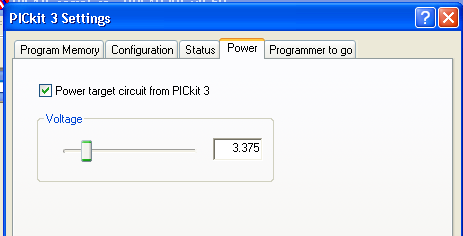
\includegraphics{phys1600/power_setting.png}
\caption{Voltage Setting Using the PICkit3 and IDE (not needed Power Lead Included)}
\label{voltagesetting}
\end{figure}

A warning message will pop up (shown in Figure~\ref{voltagecaution}). It will say the 
same thing regardless if
the voltage has been shifted down to 3.375 volts or not. The dialog box
can be moved around so check that the voltage is set to 3.375. The
checking is not essential if Pin2 of the PICkit3 is not actually
connected to anything! Click on \textbf{OK}.

\begin{figure}[htbp]
\centering
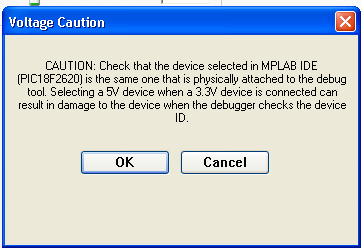
\includegraphics{phys1600/voltage_caution.png}
\caption{Warning Of Possible Voltage Issue}
\label{voltagecaution}
\end{figure}

The PICkit3 firmware progresses and says shows the \textbf{Device ID
Revision = 00000007} (see Figure~\ref{deviceid}). At this point the MPlab IDE tools for interacting
with the PIC device become visible, the tools contain color and are responsive meaning
the device can now be programmed (see Figure~\ref{programmingtools}.

\begin{figure}[htbp]
\centering
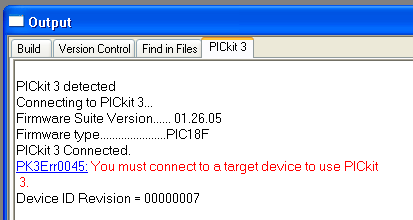
\includegraphics{phys1600/device_id.png}
\caption{Device ID Pops Up after Error Message Once the OK Button Clicked}
\label{deviceid}
\end{figure}

Once printed the error message does not go away (unless it scrolls up
out of view) but the new line with the device id is an indication that
the MPlab IDE is now talking to the PIC18LF device (still refering to Figure~\ref{deviceid}.

\begin{figure}[htbp]
\centering
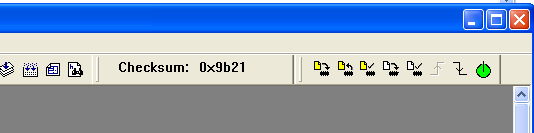
\includegraphics{phys1600/programming_tools.png}
\caption{Programming Tools Active}
\label{programmingtools}
\end{figure}

\section{For Standalone Projects}

In Phys1600 there will be some projects which are standalone. In these
cases power from a USB port will not be available and a computer will
not be available to display results. In those cases battery power will
be needed. The LCD module that we typically use requires 5 VDC (the LCD
is not required when attached to a laptop since we can run a terminal
program on the laptop).

I found a suitable DC-DC converter that can provide a regulated 5 Volts
out even when the input voltage is substantially less than 5 volts. See
\url{http://www3.telus.net/danpeirce/notes/dc_dc_converter.html}.

\section{Other things of Interest}

\subsection{TFT LCD}

4D Systems makes small TFT LCDs with full color, built-in controller,
sound, touch screen and SD-card interface. They package some in kits
complete with serial interface to a raspberry pi. The displays could
also be used with a microchip PIC.

See 4D\_LCD\footnote{\url{http://www3.telus.net/danpeirce/notes/4d_lcd.html}}

\subsection{Keypad}

I have been looking at keypads. It appears one can get much better value
purchasing a 3x4 keypad rather than a 4by4 keypad. It would actually be
cheaper to have two 3x4 keypads on a project than one 4x4 so I'd
recomend getting the 3x4. I expect the 3x4 ones are less expensive
because they are sutiable for telephones.

this one looks like a good deal from a Canadian source:

\begin{itemize}
\item
  \url{http://www.solarbotics.com/product/50847/}
\end{itemize}

\subsection{Breakout Board for SC16IS750 I2C/SPI-to-UART IC}

\href{http://www.sparkfun.com/products/9981}{Breakout Board for
SC16IS750 I2C/SPI-to-UART IC} -- while this is a real interesting little
board and one could gain an extra USART interface, it would actually
cost less and gain more functionality to connect to another PIC18LF2620!

\subsection{Breakout Board for SD-MMC Cards}

\textbf{Looks like this sparkfun breakout board has been discontinued.}
\href{http://www.sparkfun.com/products/204}{Breakout Board for SD-MMC
Cards} -- ``With SD and MMC memory prices dropping, the time is right
for mass storage and datalogging. This breakout board will allow you to
breakout the SD/MMC socket to a standard .1'' 11-pin header. Perfect for
breadboarding and the likes. Board comes fully assembled and tested as
shown." see \url{http://www.maxim-ic.com/app-notes/index.mvp/id/3969}

\url{http://www.solarbotics.com/product/13200/} \textbf{Looks like this
one costs less and has more on it (changed link as old link was broken
Nov. 21, 2012 -- nothing stands still).} Also, this is from a Canadian
source.

Links to
\url{http://site.gravitech.us/MicroResearch/Others/SD-ADP/SDmanual.pdf}

\subsection{3.3 volt 8 MHz Crystal}

\url{http://www.digikey.ca/product-detail/en/CB3LV-3C-8M0000/CTX264LVCT-ND/280258}

\begin{itemize}
\item
  \url{http://www.ctscorp.com/components/Datasheets/008-0256-0_F.pdf}
\end{itemize}

\subsection{Line in vs Mic input of PC}

\begin{itemize}
\item
  \url{http://circuits.radio-electronics.co/audio/speakers-systems/line-level-signal-to-microphone-input-adapter/}
\end{itemize}

\end{document}
